\documentclass{beamer}
\mode<presentation>
\usepackage{amsmath}
\usepackage{amssymb}
%\usepackage{advdate}
\usepackage{adjustbox}
\usepackage{subcaption}
\usepackage{enumitem}
\usepackage{multicol}
\usepackage{mathtools}
\usepackage{listings}
\usepackage{float}
\usepackage{graphicx}
\usepackage{url}
\def\UrlBreaks{\do\/\do-}
\usetheme{Boadilla}
\usecolortheme{lily}
\setbeamertemplate{footline}
{
  \leavevmode%
  \hbox{%
  \begin{beamercolorbox}[wd=\paperwidth,ht=2.25ex,dp=1ex,right]{author in head/foot}%
    \insertframenumber{} / \inserttotalframenumber\hspace*{2ex} 
  \end{beamercolorbox}}%
  \vskip0pt%
}
\setbeamertemplate{navigation symbols}{}

\providecommand{\nCr}[2]{\,^{#1}C_{#2}} % nCr
\providecommand{\nPr}[2]{\,^{#1}P_{#2}} % nPr
\providecommand{\mbf}{\mathbf}
\providecommand{\pr}[1]{\ensuremath{\Pr\left(#1\right)}}
\providecommand{\qfunc}[1]{\ensuremath{Q\left(#1\right)}}
\providecommand{\sbrak}[1]{\ensuremath{{}\left[#1\right]}}
\providecommand{\lsbrak}[1]{\ensuremath{{}\left[#1\right.}}
\providecommand{\rsbrak}[1]{\ensuremath{{}\left.#1\right]}}
\providecommand{\brak}[1]{\ensuremath{\left(#1\right)}}
\providecommand{\lbrak}[1]{\ensuremath{\left(#1\right.}}
\providecommand{\rbrak}[1]{\ensuremath{\left.#1\right)}}
\providecommand{\cbrak}[1]{\ensuremath{\left\{#1\right\}}}
\providecommand{\lcbrak}[1]{\ensuremath{\left\{#1\right.}}
\providecommand{\rcbrak}[1]{\ensuremath{\left.#1\right\}}}
\theoremstyle{remark}
\newtheorem{rem}{Remark}
\newcommand{\sgn}{\mathop{\mathrm{sgn}}}
\providecommand{\abs}[1]{\left\vert#1\right\vert}
\providecommand{\res}[1]{\Res\displaylimits_{#1}} 
\providecommand{\norm}[1]{\lVert#1\rVert}
\providecommand{\mtx}[1]{\mathbf{#1}}
\providecommand{\mean}[1]{E\left[ #1 \right]}
\providecommand{\fourier}{\overset{\mathcal{F}}{ \rightleftharpoons}}
%\providecommand{\hilbert}{\overset{\mathcal{H}}{ \rightleftharpoons}}
\providecommand{\system}{\overset{\mathcal{H}}{ \longleftrightarrow}}
	%\newcommand{\solution}[2]{\textbf{Solution:}{#1}}
%\newcommand{\solution}{\noindent \textbf{Solution: }}
\providecommand{\dec}[2]{\ensuremath{\overset{#1}{\underset{#2}{\gtrless}}}}
\newcommand{\myvec}[1]{\ensuremath{\begin{pmatrix}#1\end{pmatrix}}}
\let\vec\mathbf

\lstset{
language=C,
frame=single, 
breaklines=true,
columns=fullflexible
}

\numberwithin{equation}{section}

\title{Presentation - Matgeo}
\author{Aryansingh Sonaye \\
AI25BTECH11032 \\
EE1030 - Matrix Theory}

\date{\today} 
\begin{document}

\begin{frame}
\titlepage
\end{frame}

\section{Problem}
\begin{frame}
\frametitle{Problem Statement}
\textbf{Problem 9.4.4}

Find the roots of the following quadratic equation graphically:
\begin{align}
x^2 - 3x - 10 = 0
\end{align}


\end{frame}

\section{Solution}
\subsection{Description of Variables used}
\begin{frame}
\frametitle{Description of Variables used}
The given quadratic can be written in the conic form
\begin{align}
\vec{x}^T V \vec{x} + 2\vec{u}^T \vec{x} + f = 0
\end{align}
where
\begin{align}
V = \myvec{1 & 0 \\ 0 & 0}, \quad
\vec{u} = \myvec{-\tfrac{3}{2} \\ 0}, \quad
f = -10
\end{align}

Since the roots of the quadratic correspond to intersections with the $x$-axis, we represent the line
\begin{align}
L: \vec{x} = \vec{h} + \kappa \vec{m}
\end{align}
with
\begin{align}
\vec{h} = \myvec{0 \\ 0}, \quad
\vec{m} = \myvec{1 \\ 0}.
\end{align}

\end{frame}

\begin{frame}
\frametitle{Description of Variables used}

\begin{table}[H]
\centering
\begin{tabular}{|c|c|}
\hline
\textbf{Symbol} & \textbf{Value} \\
\hline
$V$ & $\myvec{1 & 0 \\ 0 & 0}$ \\
\hline
$\vec{u}$ & $\myvec{-\tfrac{3}{2} \\ 0}$ \\
\hline
$f$ & $-10$ \\
\hline
$\vec{h}$ & $\myvec{0 \\ 0}$ \\
\hline
$\vec{m}$ & $\myvec{1 \\ 0}$ \\
\hline
\end{tabular}
\end{table}

\end{frame}

\subsection{Theoretical Solution }
\begin{frame}
\frametitle{Theoretical Solution}
The points of intersection of a line with a conic are given by
\begin{align}
\kappa &= \frac{1}{\vec{m}^T V \vec{m}}
\Bigg(-\vec{m}^T(V\vec{h}+\vec{u}) 
\pm \sqrt{(\vec{m}^T(V\vec{h}+\vec{u}))^2 - g(\vec{h})(\vec{m}^T V \vec{m})}\Bigg),
\end{align}
where
\begin{align}
g(\vec{h}) &= \vec{h}^T V \vec{h} + 2\vec{u}^T \vec{h} + f.
\end{align}

\noindent\textbf{Step 1: Compute $m^T V m$}  
\begin{align}
\vec{m}^T V \vec{m} = \myvec{1 & 0}\myvec{1 & 0 \\ 0 & 0}\myvec{1 \\ 0} = 1
\end{align}

\end{frame}

\begin{frame}
\frametitle{Theoretical Solution}
\noindent\textbf{Step 2: Compute $Vh + u$}  
\begin{align}
V\vec{h} + \vec{u} = \myvec{0 \\ 0} + \myvec{-\tfrac{3}{2} \\ 0} = \myvec{-\tfrac{3}{2} \\ 0}
\end{align}

\noindent\textbf{Step 3: Compute $m^T(Vh+u)$}  
\begin{align}
\vec{m}^T(V\vec{h}+\vec{u}) = \myvec{1 & 0}\myvec{-\tfrac{3}{2} \\ 0} = -\tfrac{3}{2}
\end{align}

\noindent\textbf{Step 4: Compute $g(h)$}  
\begin{align}
g(\vec{h}) = \vec{h}^T V \vec{h} + 2\vec{u}^T \vec{h} + f = -10
\end{align}

\end{frame}

\begin{frame}
\frametitle{Theoretical Solution}
\noindent\textbf{Step 5: Substitute into formula for $\kappa$}  
\begin{align}
\kappa &= -(-\tfrac{3}{2}) \pm \sqrt{\left(-\tfrac{3}{2}\right)^2 - (-10)(1)} \\[1ex]
&= \tfrac{3}{2} \pm \sqrt{\tfrac{9}{4} + 10} \\[1ex]
&= \tfrac{3}{2} \pm \sqrt{\tfrac{49}{4}} \\[1ex]
&= \tfrac{3}{2} \pm \tfrac{7}{2}
\end{align}

\noindent\textbf{Step 6: Evaluate roots}  
\begin{align}
\kappa_1 &= \tfrac{3}{2} + \tfrac{7}{2} = 5 \\
\kappa_2 &= \tfrac{3}{2} - \tfrac{7}{2} = -2
\end{align}


\end{frame}

\begin{frame}
\frametitle{Theoretical Solution}
\noindent\textbf{Step 7: Find intersection points}  
The intersection points are obtained as
\begin{align}
\vec{x}_1 &= \vec{h} + \kappa_1 \vec{m} 
= \myvec{0 \\ 0} + 5\myvec{1 \\ 0} = \myvec{5 \\ 0} \\[1ex]
\vec{x}_2 &= \vec{h} + \kappa_2 \vec{m} 
= \myvec{0 \\ 0} - 2\myvec{1 \\ 0} = \myvec{-2 \\ 0}
\end{align}

\section*{Final Answer}

Thus, the quadratic $x^2 - 3x - 10 = 0$ intersects the $x$-axis at
\begin{align}
\boxed{x = -2 \quad \text{and} \quad x = 5}
\end{align}


\end{frame}


\subsection{Plot}
\begin{frame}
    \frametitle{Plot}
\begin{figure}[H]
   \centering
   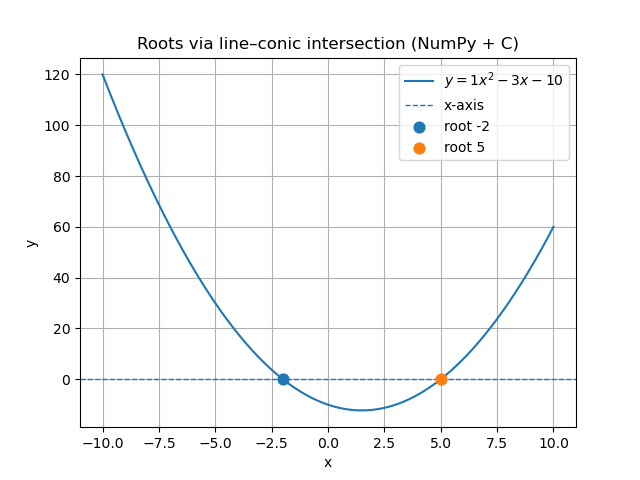
\includegraphics[width=0.8\columnwidth]{figs/parabola.png}
   \caption{}
   \label{}
   \end{figure}
\end{frame}

\begin{frame}[fragile]
    \frametitle{Code - C}
    \begin{lstlisting}
#include <math.h>

void intersect_line_conic(
    const double V[4],     // 2x2 row-major: [V00,V01,V10,V11]
    const double u[2],     // size-2
    double f,              // scalar
    const double h[2],     // line anchor
    const double m[2],     // line direction
    double kappa_out[2],   // outputs
    double x1[2],
    double x2[2],
    int *status            // 2=two real, 1=one (tangent), 0=none
) {
    double Vm0 = V[0]*m[0] + V[1]*m[1];
    double Vm1 = V[2]*m[0] + V[3]*m[1];
    double mTVm = m[0]*Vm0 + m[1]*Vm1;


    \end{lstlisting}
    \end{frame}

    \begin{frame}[fragile]
    \frametitle{Code - C}
    \begin{lstlisting}
    double Vh0 = V[0]*h[0] + V[1]*h[1];
    double Vh1 = V[2]*h[0] + V[3]*h[1];

    double Vh_u0 = Vh0 + u[0];
    double Vh_u1 = Vh1 + u[1];

    double mT_Vh_u = m[0]*Vh_u0 + m[1]*Vh_u1;

    double hTVh = h[0]*Vh0 + h[1]*Vh1;
    double two_uTh = 2.0*(u[0]*h[0] + u[1]*h[1]);
    double g = hTVh + two_uTh + f;

    double disc = mT_Vh_u*mT_Vh_u - g*mTVm;


    \end{lstlisting}
    \end{frame}

        \begin{frame}[fragile]
    \frametitle{Code - C}
    \begin{lstlisting}
    if (disc > 1e-12) {
        double r = sqrt(disc);
        kappa_out[0] = (-mT_Vh_u + r) / mTVm;
        kappa_out[1] = (-mT_Vh_u - r) / mTVm;
        x1[0] = h[0] + kappa_out[0]*m[0];  x1[1] = h[1] + kappa_out[0]*m[1];
        x2[0] = h[0] + kappa_out[1]*m[0];  x2[1] = h[1] + kappa_out[1]*m[1];
        *status = 2;
    } else if (fabs(disc) <= 1e-12) {
        kappa_out[0] = kappa_out[1] = (-mT_Vh_u) / mTVm;
        x1[0] = x2[0] = h[0] + kappa_out[0]*m[0];
        x1[1] = x2[1] = h[1] + kappa_out[0]*m[1];
        *status = 1;
    } else {
        *status = 0;}
}


    \end{lstlisting}
    \end{frame}

\begin{frame}[fragile]
    \frametitle{Code - Python(with shared C code)}
    The code to obtain the required plot is
    \begin{lstlisting}
import ctypes as ct
import numpy as np
import matplotlib.pyplot as plt
# --- load the shared library (same folder) ---
lib = ct.CDLL("./libsimple_conic.so")
# tell ctypes what arguments the C function expects
lib.intersect_line_conic.argtypes = [
    ct.POINTER(ct.c_double),  # V[4]
    ct.POINTER(ct.c_double),  # u[2]
    ct.c_double,              # f
    ct.POINTER(ct.c_double),  # h[2]
    ct.POINTER(ct.c_double),  # m[2]
    ct.POINTER(ct.c_double),  # kappa[2] out
    ct.POINTER(ct.c_double),  # x1[2] out
    ct.POINTER(ct.c_double),  # x2[2] out
    ct.POINTER(ct.c_int)      # status out

\end{lstlisting}
\end{frame}
\begin{frame}[fragile]
\frametitle{Code - Python(with shared C code)}
\begin{lstlisting}
]
lib.intersect_line_conic.restype = None

# ---- helper: convert quadratic ax^2+bx+c into conic form ----
def quadratic_to_conic(a, b, c):
    V = np.array([a, 0.0, 0.0, 0.0], dtype=np.double)     # [[a,0],[0,0]]
    u = np.array([b/2.0, 0.0], dtype=np.double)           # so 2u^T x = b x
    f = np.double(c)
    return V, u, f

# ---- our quadratic: x^2 - 3x - 10 = 0 ----
a, b, c = 1.0, -3.0, -10.0
V, u, f = quadratic_to_conic(a, b, c)

# Intersect with x-axis (y=0): line x = h + k m
h = np.array([0.0, 0.0], dtype=np.double)
m = np.array([1.0, 0.0], dtype=np.double)



\end{lstlisting}
\end{frame}

\begin{frame}[fragile]
\frametitle{Code - Python(with shared C code)}
\begin{lstlisting}
# Outputs (allocated for C)
kappa = np.zeros(2, dtype=np.double)
x1 = np.zeros(2, dtype=np.double)
x2 = np.zeros(2, dtype=np.double)
status = ct.c_int(0)
# ---- call the C function ----
lib.intersect_line_conic(
    V.ctypes.data_as(ct.POINTER(ct.c_double)),
    u.ctypes.data_as(ct.POINTER(ct.c_double)),
    ct.c_double(f),
    h.ctypes.data_as(ct.POINTER(ct.c_double)),
    m.ctypes.data_as(ct.POINTER(ct.c_double)),
    kappa.ctypes.data_as(ct.POINTER(ct.c_double)),
    x1.ctypes.data_as(ct.POINTER(ct.c_double)),
    x2.ctypes.data_as(ct.POINTER(ct.c_double)),
    ct.byref(status)
)


\end{lstlisting}
\end{frame}

\begin{frame}[fragile]
\frametitle{Code - Python(with shared C code)}
\begin{lstlisting}
# Collect results
roots = []
if status.value >= 1:
    roots.append(float(x1[0]))
    if status.value == 2:
        roots.append(float(x2[0]))
roots.sort()
print("status:", status.value)
print("roots:", roots)  # expected [-2.0, 5.0]

# ---- plot parabola and roots ----
xs = np.linspace(-10, 10, 600)     # simpler fixed range
ys = a*xs*xs + b*xs + c



\end{lstlisting}
\end{frame}

\begin{frame}[fragile]
\frametitle{Code - Python(with shared C code)}
\begin{lstlisting}
plt.figure()
plt.plot(xs, ys, label=rf"$y={a:.0f}x^2{b:+.0f}x{c:+.0f}$")
plt.axhline(0, linestyle="--", linewidth=1, label="x-axis")
for r in roots:
    plt.scatter([r], [0.0], s=60, zorder=3, label=f"root {r:g}")
plt.xlabel("x"); plt.ylabel("y")
plt.title("Roots via line-conic intersection (NumPy + C)")
plt.grid(True)
plt.legend()
plt.savefig("parabola.png")
plt.show()


\end{lstlisting}
\end{frame}



\begin{frame}[fragile]
\frametitle{Code - Python only}
\begin{lstlisting}
import numpy as np
import matplotlib.pyplot as plt

# ---------- Helpers ----------

def quadratic_to_conic(a, b, c):
    V = np.array([[a, 0.0],
                  [0.0, 0.0]], dtype=float)
    u = np.array([b/2.0, 0.0], dtype=float)   # so that 2 u^T x = b x
    f = float(c)
    return V, u, f

def line_conic_intersection(V, u, f, h, m, eps=1e-12):
    # m^T V m
    Vm = V @ m
    mTVm = float(m @ Vm)


\end{lstlisting}
\end{frame}

\begin{frame}[fragile]
\frametitle{Code - Python only}
\begin{lstlisting}
    # Vh + u
    Vh_u = V @ h + u
    # m^T (Vh + u)
    mT_Vh_u = float(m @ Vh_u)
    # g(h) = h^T V h + 2 u^T h + f
    g = float(h @ (V @ h) + 2.0 * (u @ h) + f)
    disc = mT_Vh_u**2 - g * mTVm
    if disc > eps:
        r = np.sqrt(disc)
        k1 = (-mT_Vh_u + r) / mTVm
        k2 = (-mT_Vh_u - r) / mTVm
        X1 = h + k1 * m
        X2 = h + k2 * m
        return 2, np.array([k1, k2], dtype=float), np.vstack([X1, X2])


\end{lstlisting}
\end{frame}

\begin{frame}[fragile]
\frametitle{Code - Python only}
\begin{lstlisting}
    elif abs(disc) <= eps:
        k = (-mT_Vh_u) / mTVm
        X = h + k * m
        return 1, np.array([k, k], dtype=float), np.vstack([X, X])
    else:
        return 0, np.array([np.nan, np.nan]), np.array([[np.nan, np.nan],
                                                        [np.nan, np.nan]])

# ---------- Problem setup ----------

# Given quadratic: x^2 - 3x - 10 = 0
a, b, c = 1.0, -3.0, -10.0

# Conic parameters (V, u, f)
V, u, f = quadratic_to_conic(a, b, c)

\end{lstlisting}
\end{frame}

\begin{frame}[fragile]
\frametitle{Code - Python only}
\begin{lstlisting}
# x-axis as the line: y = 0  -> h = (0,0), m = (1,0)
h = np.array([0.0, 0.0], dtype=float)
m = np.array([1.0, 0.0], dtype=float)

# ---------- Solve via line-conic intersection ----------
status, kappa, X = line_conic_intersection(V, u, f, h, m)

# Roots are the x-coordinates of intersection points with y=0
roots = []
if status >= 1:
    roots = sorted([float(X[0, 0]), float(X[1, 0])]) if status == 2 else [float(X[0, 0])]

print("Status (2:two real, 1:tangent, 0:none):", status)
print("kappa values:", kappa)
print("Intersection points (x,y):\n", X)
print("Roots (x-intercepts):", roots)


\end{lstlisting}
\end{frame}

\begin{frame}[fragile]
\frametitle{Code - Python only}
\begin{lstlisting}
# ---------- Plot ----------
xs = np.linspace(-10, 10, 600)
ys = a*xs**2 + b*xs + c

plt.figure()
plt.plot(xs, ys, label=rf"$y={a:.0f}x^2{b:+.0f}x{c:+.0f}$")
plt.axhline(0, linestyle="--", linewidth=1, label="x-axis")

if status >= 1:
    plt.scatter([X[0,0]], [0.0], s=60, zorder=3, label=f"root {X[0,0]:g}")
    if status == 2:
        plt.scatter([X[1,0]], [0.0], s=60, zorder=3, label=f"root {X[1,0]:g}")
 

\end{lstlisting}
\end{frame}

\begin{frame}[fragile]
\frametitle{Code - Python only}
\begin{lstlisting}
plt.xlabel("x"); plt.ylabel("y")
plt.title("Roots via line-conic intersection (vectors & matrices)")
plt.grid(True)
plt.legend()
plt.savefig("newparabola.png")
plt.show()
 
 

\end{lstlisting}
\end{frame}

\end{document}
